%****************************************************
%	CHAPTER 3 - Design Methodology
%****************************************************

\chapter{Design methodology}
\label{ch:ch3}
\section{Design overview}
\label{sec:ch3_design}

In Chapter \ref{ch:chapter2}, the critical areas, challenges and techniques used by remote sensing devices to meet the objectives outlined in \ref{sec:ch1.section1} were discussed.  Remote sensing devices aim to increase the temporal and spatial resolution of Southern Ocean data sets by increasing survivability and concentration of remote sensing platforms. The challenges identified in Chapter \ref{ch:chapter2} were the sea ice dynamics which can damage the device. Furthermore, strong wave activity and low temperatures which can freeze the device and degrade the battery life. A key difference between each device was the measurement objectives as shown in Table \ref{tab:device_deployment} which dictated the sensors, processing strategy and functionality of each system. \par

This section outlines the steps taken to identify the user requirements and translate them into hardware subsystems. The design phase began with a user requirements analysis. These requirements resulted in well-defined measurement objectives for the device and the selection of subsystems critical to the device functions. Then, a high-level system diagram was created to show the interaction of the subsystems within the system. This allowed for the selection of hardware components to satisfy the requirements for each subsystem. Finally, to ensure that the subsystems met the user requirements, a set of acceptance tests were derived. 


\section{User Requirements}
\label{sec:sec3_UR}

The user requirements analysis began with an identification of the project stakeholders shown in Appendix \ref{app:stakeholder}. Through constant engagement with the primary stakeholders, a set of user requirements was generated which identified the objectives the device would need to meet. The formatting, presentation and selection of these user requirements was done in accordance with IEEE Standards\footcite{IEEE_STD_UREQ}

\begin{table}[H]
    \centering
        \caption{User requirements obtained by meeting with the principal stakeholders. These will be used to determine the desired functionality of the buoy}
        \setlength{\extrarowheight}{5pt}
        \resizebox{\textwidth}{!}{%
    \begin{tabular}{ >{\centering\arraybackslash} m{0.3\textwidth}  >{\raggedright\arraybackslash} m{0.7\textwidth} }
    \hline
       \textbf{User Requirement ID}  & \textbf{Description}  \\
       \hline
       \hline
       UR001  & System must be able to withstand the Southern Ocean climate.\\
       \hline
       UR002 & System must be able to transmit data remotely without additional infrastructure or user input. \\
       \hline
       UR003 & System shall provide higher temporal and spatial resolution data. \\
       \hline
       UR004 & System must be capable of measuring  ice floe dynamics and environmental conditions surrounding sea ice formation. \\
       \hline
       UR005 & System must be user-friendly and easy to deploy.\\
       \hline
       UR006 & System Must be cost effective. \\
       \hline
       UR007 & System must be able to store and process data in an organised manner. \\
       \hline
    \end{tabular}}

    \label{tab:user_reqs}
\end{table}

\subsection{Analysis of UR001}
\textit{System must be able to withstand the Southern Ocean climate.}

\textcite{kohout2015device} encountered 7 m swell and 25 $\text{ms}^{-1}$ winds during their deployment in the marginal ice zone which lead to the immediate failure of one of their systems \cite{kohout2015device}. Strong wind and waves were also observed by \textcite{vichi2019effects,alberello2019drift} during their deployment which has been attributed to multiple cyclonic events coinciding with the deployment of the WIIOS buoys. The effects of wind and waves result in the delay of consolidation of sea ice at the edge of the marginal ice zone  which created survivability challenges for the devices. Additionally, \textcite{albarello2020drift} showed that wind speed resulted in ice floe drifting at $0.35$ $\text{ms}^{-1}$. Placing the buoy close to the surface of the ice subjects it to collisions, breaking and rafting which resulted in the failures of \cite{doble2017robust,rabault2019open}. Snow and ice formation on the surface of the floe can bury the device \cite{doble2017robust}  and constant wave energy on unconsolidated ice cause flooding which can further damage the devices. A device that is elevated above the surface while tethered to the floe can reduce exposure to these events however the buoy elevation must be at least 1 m to compensate for snow growth \cite{barber2005microwave}. \par

Furthermore, for a device to survive in the Southern Ocean, the software must contain a robust set of error checking for each module. The software should ensure that critical subsystems are functional and responsive while constantly providing feedback on statuses. Should a module be damaged or go offline, the software should flag this issue, identify the failure and attempt to rectify it. Alternatively, if the failure is critical, the device should flag the module as malfunctioning and continue to operate without it.

\subsection{Analysis of UR002}
\textit{System must be able to transmit data remotely without additional infrastructure or user input.}

\textcite{kennicutt2016delivering} shows a fundamental lack of infrastructure on the Antarctic continent including data networks. Operations taking place on sea ice are isolated from any resources that exist via Antarctic bases. Sea ice in the marginal ice zone is subject to conditions inhospitable to humans \cite{kennicutt2016delivering}. Therefore access to the buoys is limited once the device is deployed often making it difficult to retrieve. The life cycle of sea ice presents an additional access challenge through the consolidation of sea ice  during the freezing periods and melting  of the ice floes during the warming periods \cite{womack_2020}. Additionally, manned expeditions are typically inflexible \cite{kennicutt2016delivering} resulting in additional challenges in retrieving the buoy and hence the data. Therefore, most devices deployed in the region are designed to be expendable (\cite{kohout2015device,rabault2019open,trident}). These device circumvent this by using satellite networks with global coverage such as Iridium\footnote{See Chapter \ref{ch2:secdevice}} which allows the users to receive data and status updates from the buoy without needing to retrieve the devices. 

The lack of user input implies that device routines and sub routines must be performed automatically. The device should control and sample sensors in a fixed, predictable manner ensuring that the correct data is sampled during the correct periods. Furthermore, the device needs to transmit data over the Iridium network. Therefore the software is required to control the interactions with the mode ensuring that it is functional. The software should condense data to fit the bandwidth of the device and ensure it is successfully uploaded to the transmission buffer. Finally, the software should be able to check for sufficient network availability and initiate a transmission. Should an error occur, the software needs to respond and handle it efficiently.

\subsection{Analysis of UR003}
\textit{System shall provide higher temporal and spatial resolution data.}

Phases of the sea ice life cycle are defined by periods of freezing followed by periods of melting \cite{barber2005microwave} with maximum extents occurring in winter (freezing) and summer (melting) respectively \cite{barber2005microwave}. The formation and consolidation of sea ice floes are influenced by atmospheric and oceanic processes resulting in the delay of sea ice consolidation \cite{vichi2019effects,albarello2020drift}. Each period coincides with a seasonal cycle typical lasting a few months \cite{vichi2019effects,alberello2019drift,barber1948generation} which is the length of time a buoy needs to survive to provide sufficient data on a temporal scale. \par 

Increasing remote sensing in the region is also required to provide spatial coverage \cite{albarello2020drift}. Certain observational methods such as satellite observation are performed on a 10 m scale \cite{galin2011validation} where sea ice variability can scale down to the cm \cite{vichi2019effects}. \textcite{doble2017robust} achieved large spatial coverage by deploying the devices in clusters of five every 5 km. Additional deployments from \cite{vichi2019effects}, \cite{kohout2015device} and \cite{albarello2020drift}
also achieved this by deploying multiple systems spaced 3 to 4 m apart \cite{vichi2019effects}. Therefore increasing the spatial resolution can be achieved by increasing the concentration of devices in an area spaced apart. \par 

For a remote sensing device to survive the required period, a built-in power source is required to maintain functionality without constant maintenance. This power supply primarily needs to come from a replenishable source. \textcite{doble2017robust} and \textcite{rabault2019open} coupled battery arrays to a rechargeable power system which showed promise however, insufficient cloud cover \cite{doble2017robust} resulted in the solar panel being underutilised. As discussed in Chapter \ref{ch:chapter2}, commercial batteries are readily available and well-specified to supply power for long periods \cite{rabault2017measurements}. However, the system must conserve energy. Otherwise, this could result in low survival rates \cite{kohout2015device}. Additionally, batteries in sub-zero temperatures have a significantly reduced capacity of up to 50\% \cite{doble2017robust}.

Therefore, the software needs to contain power monitoring capabilities. A sensor should monitor the current and power usage of the device and provide feedback to the system. The device software should be optimized to conserve power which means turning off sensors that are not in use and entering low power mode during periods of inactivity. Finally, the software needs to handle power events that could disrupt the functionality of the buoy such as brownouts and power resets. The software should be able to recognize when the power is too low to operate and respond accordingly.

\subsection{Analysis of UR004}

\textit{System must be capable of measuring ice floe dynamics and environmental conditions surrounding sea ice formation.}

As discussed in Chapter \ref{ch2:secdevice}, in situ, remote sensing devices have been deployed in the Southern Ocean with specific measurement objectives. Table \ref{tab:device_deployment} shows that the following measurements were common to one or more devices:
\begin{itemize}
	\item Ice drift
	\item Collisions between ice floes
	\item Waves in ice
	\item Ambient temperature
	\item Atmospheric pressure
\end{itemize}

\subsubsection{Meteorological sensing requirements}

Temporal resolutions and measurement standards need to be taken in accordance with the World Meteorological Organisation to ensure effective communication and standardisation of the data sets \cite{worldmeteorologicalorganization_2010}. For environmental data and wave spectra, the data are provided in Table \ref{tab:metocean} below:

\begin{table}[H]
	\centering
	\caption{Comparison of standard measurements for meteorological data including temporal resolution, measurement unit and accuracy from: \cite{worldmeteorologicalorganization_2010}}
	\setlength{\extrarowheight}{5pt}
	\begin{tabular}{lll}
		\hline
		\textbf{Variable Name}  & \textbf{Resolution} & \textbf{Accuracy}\\
		\hline
		\hline
		Temperature & 1 hour & $\pm$0.5 K \\
		
		Pressure & 1 hour & $\pm$ 0.5 HPa \\
		
		Wind Speed & 1 hour & $\pm \text{2 ms}^{-1}$\\
		\hline
	\end{tabular}
	\label{tab:metocean}
\end{table}

Meteorological data should be sampled from a height of 1 to 40 m  \cite{worldmeteorologicalorganization_2010}. Therefore, all meteorological sensors should be mounted 1 m above the ground to meet these standards. Additionally, the software should be capable of retrieving data from a temperature and pressure sensor. The software should also contain error checking to ensure robust sampling and reliable data from the sensors. \par 

\subsubsection{Ice drift sensing requirements}

\textcite{trident,uptempo,kohout2015device} and \textcite{albarello2020drift} show that ice drift measurements can be taken using a GNSS tracker can be used to monitor by recording the global coordinates against an accurate time reference. \textcite{alberello2019drift} show that temporal resolutions affect the behaviour of drift data. Devices that went into low power mode during deployment (\cite{vichi2019effects,alberello2019drift}) had decreased sampling rates which failed to capture ice drift oscillations. \textcite{albarello2020drift} further show that a temporal resolution of 3 hours is required to capture ice drift oscillations. Additionally, the GPS reading can be affected by the number of satellites picked up by the receiver (dependent on the receiver antenna gain) \cite{spilker1996global}, the spread of satellites and the angle of elevation above the horizon. A characteristic of this error is called the dilution of precision (DOP). This value details the positional or temporal measurement inaccuracy. Moreover, the software needs to accommodate a GPS module and interface with it through a suitable communication port. The software needs to sample the GPS at a frequency of once every 3 hours or less. Finally, the software should configure the GPS module to transmit diagnostic information, positional error and temporal error information in addition to time and date information.\par 

\subsubsection{Waves in ice sensing requirements}

Wave in ice measurements play a critical role in understanding the formation of sea ice in the marginal ice zone \cite{alberello2019drift}. Low frequency, high energy waves propagate through the area and displace the ice floes \cite{womack_2020}. Current devices such as those developed by \cite{rabault2017measurements,thomson2012wave,kohout2015device} utilise either a statistical \cite{kuik1988method} or spectral \cite{earle1996nondirectional,welch1967use} approach which allows for measurements of waves independent of the dynamics of the ice floe. These methods require roll, heave, pitch and vertical acceleration measurements for 1000 s at sample rates above 0.5 Hz, which corresponds to the upper band of ocean waves \cite{earle1996nondirectional}. The software should be capable of interfacing with an IMU and should ensure that data is sampled at a fixed sample rate for the required period. The software should also store the data in an area with sufficient space. Finally, the software should contain error checking algorithms to ensure robust communication with this device. \par 

\subsection{Analysis of UR005}

\textit{System must be  user-friendly and easy to deploy}

Table \ref{tab:device_price} shows the weight of each system. Notably, the lightest device being the Trident buoy at 0.42 kg and the heaviest being the buoys by \textcite{doble2017robust}. The weight of the device significantly affects the deployment protocol. Heavy devices will require a large team to deploy the device and specialised courier methods to transport it such as those described in \textcite{doble2017robust}. Devices that weighed 4.5 kg to 30 kg were light enough to be carried by one person and deployed much faster.

The deployment is also affected by the set up of the device. The SIMB Buoy, while being relative light, requires a team to assemble the components on the ice and drill a hole to place it in \cite{PLANCK2019102792}. \textcite{kennicutt2016delivering} shows that certain polar regions are too dangerous for manned missions, which can limit the deployment location and time frame the crew can spend setting up the buoy. However, systems that are relatively easy to deploy (Trident, WIIOS, SWIFT) allow for sensing near dangerous environments such as the ice edge of the marginal ice zone. These devices are preassembled and set up leading to a "drop and go" style deployment from ship cranes \cite{vichi2019effects,alberello2019drift} or boats \cite{rabault2019open,kohout2015device}. The software should be configured to begin execution as soon as the device is operational. Software settings and parameters should be loaded into permanent storage and the sensors should be calibrated before being sent on the expeditions.

\subsection{Analysis of UR006}

\textit{System must be cost effective}

\textcite{PLANCK2019102792,guimaraes2018surface,rabault2019open} consider cost to be a significant constraint in designing a system. Additionally, some devices such as SIMB buoy, gradually factored in price after two iterations \cite{planck2019evolution}. This shows that optimising device performance for cost is critical for increasing the affordability and availability of devices. An affordable system Table \ref{tab:device_price} showed a comparison of reported costs and wughts for each system where applicable.
 
from Table \ref{tab:device_price} we can see from the cost breakdown that \textcite{rabault2019open} succeeded in creating a low cost buoy through the use of open source hardware and off-the-shelf components resulting in this device having the lowest reported price out of all the system. The next cheapest device is the Trident buoy which is only R300.00 more expensive than the WIIB. However, this device contains fewer sensors and is only capable sea ice drift and temperature measurements. On average, commercial systems (UptempO, Polar ISVP, Trident) proved to be significantly more expensive than research devices with similar attributes. However, due to the absence of prices for SWIFT, WIIOS and Trident it is difficult to draw conclusions from this comparison. Furthermore, commercial systems had design capabilities to design and print custom circuit boards and chip sets while research systems (SWIFT, WIIB, WIIOS) did not have such capabilities. Therefore, the developers optimised for procurement time by using off the shelf components \cite{kohout2015device,rabault2019open}. A novel sensing device that is cost optimized should result in an overall cost cheaper than the devices in table \ref{tab:device_price} with comparable performance, this will also allow for quicker and cheaper device procurement allowing for more devices to be produced for deployment thereby allowing for a larger spatial area in the marginal ice zone to be covered.

\subsection{Analysis of UR007}

\textit{System must be able to store and process data in an organised manner}

The proposed system will require multiple subsystems to satisfy the user requirement UR004. These subsystems will generate large volumes of data that needs to be stored and organised efficiently. As shown in the discussions for user requirements UR001 to UR005, the system will require multiple sensors and modules. Each module has different operational and communication requirements. Therefore, a suitable processor needs to be selected to provide sufficient ports to interface with each sensor. This processor should accommodate sufficiently high volumes of data with a wide enough byte size to accept sensor data without calculation errors. The software will need to meet the requirements of each sensor and sequence these functions into a routine. This can be achieved by developing sensor libraries for each device. Included in these libraries will be initialisation routines, peripheral communication drivers and sensor sampling routines to meet the requirements for each sensor. Furthermore, as shown in the discussion above, each sensing activity is time-critical. This places a strict timing requirement on the device to ensure the integrity of the data set on a temporal scale. Therefore, an accurate timing reference is required in the form of a real-time clock (RTC). \par 

Additionally, Each sensor has a different data rate requirement. Some sensors will need to stream large volumes of data of an unknown length. To deal with this, efficient data acquisition techniques need to be implemented by the software to accommodate these volumes. Such techniques include setting up direct memory access (DMA) channel in a circular buffer to stream data to a memory location with an input capture timer on slave reset mode to close the channel when the data stream is completed.\par 

Finally, long periods of inactivity between measurements can result in wasted power. The discussion of user requirement UR003 showed that the software should turn the device off or into low power mode during these periods. If the data is in the processor memory when the device is off, it could get lost. Therefore, a permanent storage device is required to store data during these periods of inactivity. The software should include functions to read from the storage space and write to it efficiently. Additional error checks should be written to ensure the storage device is online, operational and the data has not been corrupted.

Finally, the aforementioned hardware and software modules need to be verified with a suite of acceptance tests to ensure that all the user requirements have been met. 


\section{Functional requirements}
\label{sec:ch3_FR}
Analysis of the aforementioned user requirements resulted in the procurement of a set of functional requirements that dictate how the buoy will function.

\subsection{Operational requirements }

\begin{table}[H]
    \centering
    \caption{Requirements addressing the mechanical needs for the system during operation.}
    \setlength{\extrarowheight}{5pt}
    \resizebox{\textwidth}{!}{%
    \begin{tabular}{>{\centering\arraybackslash}m{0.2\textwidth}>{\RaggedRight}m{0.7\textwidth} >{\RaggedRight}m{0.25\textwidth}}
    \hline
         \textbf{Requirement ID} & \textbf{Description} & \textbf{User requirements addressed}\\
         \hline
         \hline
         \multirow{2}{0.2\textwidth}{FR001} & \multirow{2}{0.7\textwidth}{The System shall have a protective enclosure against precipitation and frost.} & UR001\\ &&UR005 \\
         \hline
         \multirow{2}{0.2\textwidth}{FR002} & \multirow{2}{0.7\textwidth}{The enclosure shall be constructed from strong, corrosion resistant materials with strong thermal characteristics.} &  UR001 \\ && UR005 \\
         \hline
         \multirow{1}{0.2\textwidth}{FR003}& The device will protect electronics from internal humidity. & UR001\\
         \hline 
          \multirow{2}{0.2\textwidth}{FR004}& \multirow{2}{0.7\textwidth}{The electronics will be elevated above the ground by 1 m.} & UR001\\ &&UR005 \\
         \hline
         \multirow{2}{0.2\textwidth}{FR005} & \multirow{2}{0.7\textwidth}{All subsystems shall be rated for extreme temperatures.} & UR001\\ && UR003\\
         \hline
         \hline
    \end{tabular}}

    \label{tab:hard_funcreqsl}
\end{table}

\subsection{Electronic requirements}

\begin{table}[H]
    \centering
    \caption{Requirements addressing the electronic needs for the system including the modules, components and sensors that satisfy the user requirements.}
    \setlength{\extrarowheight}{5pt}
    \resizebox{\textwidth}{!}{%
    \begin{tabular}{>{\centering}m{0.2\textwidth}>{\RaggedRight}m{0.7\textwidth} >{\RaggedRight}m{0.25\textwidth} }
    \hline
         \textbf{Requirement ID} & \textbf{Description} & \textbf{User requirements addressed}\\
         \hline
         \hline
         \multirow{1}{0.2\textwidth}{FR006} & System will transmit data via Iridium satellite network. & UR002\\
         \hline
         \multirow{2}{0.2\textwidth}{FR007} & \multirow{2}{0.7\textwidth}{Device shall be battery powered.} & UR001 \\ && UR003\\
         \hline
         \multirow{1}{0.2\textwidth}{FR008} & System shall measure ice drift using a  global positioning system (GPS). & UR004\\
         \hline
          \multirow{1}{0.2\textwidth}{FR009}& Device shall measure ambient temperature. & UR004\\
         \hline
         \multirow{1}{0.2\textwidth}{FR010} & Device shall measure atmospheric pressure & UR004 \\
         \hline
        \multirow{1}{0.2\textwidth}{FR011}  & Device shall contain an inertial measurement unit (IMU) to record acceleration (3-axes) and rotation (3-axes) of an ice floe. & UR004 \\
         \hline
         \hline
    \end{tabular}}
    \label{tab:other_funcreqs}
\end{table}

\subsection{Software requirements}

\begin{table}[H]
    \centering
    \caption{Software functional requirements for the system addressing the system function, performance, operation and control during the lifetime of the device.}
        \setlength{\extrarowheight}{5pt}
    \resizebox{\textwidth}{!}{%
    \begin{tabular}{>{\centering}m{0.2\textwidth}>{\RaggedRight}m{0.7\textwidth} >{\RaggedRight}m{0.25\textwidth} }
    \hline
        \textbf{Requirement ID} & \textbf{Description} & \textbf{User requirements addressed}\\
         \hline
         \hline
        \multirow{2}{0.2\textwidth}{FR012} &  \multirow{2}{0.7\textwidth}{Device to contain sufficient memory for data storage.} & UR006\\ && UR007 \\
         \hline
        \multirow{2}{0.2\textwidth}{FR013} &  \multirow{2}{0.7\textwidth}{Device to contain a processing unit to control sensors and process data.} & UR006\\ && UR007\\
         \hline
         \multirow{3}{0.2\textwidth}{FR014} &  \multirow{3}{0.7\textwidth}{Device to be optimised for low-power consumption and power event handling.} & UR003\\&& UR006 \\&& UR007  \\
         \hline
         \hline
    \end{tabular}}
    \label{tab: soft_funcreqsl}
\end{table}

\subsection{Other requirements}
\begin{table}[H]
    \centering
    \caption{ Other system requirements being addressed.}
   \setlength{\extrarowheight}{5pt}
\resizebox{\textwidth}{!}{%
	\begin{tabular}{>{\centering}m{0.2\textwidth}>{\RaggedRight}m{0.7\textwidth} >{\RaggedRight}m{0.25\textwidth} }
		\hline
		\textbf{Requirement ID} & \textbf{Description} & \textbf{User requirements addressed}\\
    \hline
    \hline
   \multirow{1}{0.2\textwidth}{FR015} & Device shall be calibrated prior to shipping and delivered in a state where it can be deployed at a moment's notice & UR005 \\
    \hline
   \multirow{1}{0.2\textwidth}{FR016} & The Device will cost less than currently available systems. & UR006 \\
    \hline
    \hline
    \end{tabular}}
    \label{tab:elec_funcreqs}
\end{table}

\section{System overview}
\label{sec:ch3_sysoverview}
To meet the functional requirements, the overall system was designed using a top down approach. The requirements highlighted in Tables \ref{tab:hard_funcreqsl} to \ref{tab:other_funcreqs} will be used to identify key subsystems to achieve the required functionality.

\begin{table}[H]
    \centering
    \caption{Table showing the subsystems that are critical to the functionality of the buoy and the level of importance indicated by rank}
    \setlength{\extrarowheight}{2.5pt}
    \begin{tabular}{l c }
    \hline
    \textbf{Name}  & \textbf{Rank}\\
    \hline
    \hline
    Firmware & 1\\
    \hline
    Power system & 2 \\
    \hline
    Communication module  & 3\\
    \hline
    Processor & 4\\
    \hline
    Sensors & 5\\
    \hline
    Permanent storage  & 6 \\
    \hline
    Mechanical features & 7 \\
    \hline
    \hline
    \end{tabular}

    \label{tab:subsys}
\end{table}

The firmware is the most critical subsystem in the device and ranks the highest in terms of priority. The firmware is crucial for the operation of the device and to control all the modules. The next most critical component is the power system. Any failures in the power system will cause the device to stop functioning.  All device components need to be rated for subzero operation to ensure robust operation. A voltage regulator will be included to ensure a constant voltage. Finally, a power sensor will be included to monitor the batteries and warn the system when the batteries are almost depleted. \par 

After the power system is the communication subsystem as Iridium will be used to transmit the data obtained by the system. Should this device fail, the device will be unable to transmit data unless it is retrieved. Satellite communication for Iridium is performed using a satellite mode while GPS communication is performed using a GPS receiver. They require, clear, unobstructed views of the satellites which can be achieved with high-gain antennas. These devices need to mounted as close to the sky as possible.\par

The sensors are the primary interface between the system and the environment. The electronics need to be as close to the exterior of the system as possible to measure ambient temperature and pressure. The IMU can be mounted anywhere inside the buoy however, the device needs to be calibrated for its position on the buoy as well as its orientation inside. \par

The sensors will interface with a central processing system which will control the sensors and sample data from them. Data coming from the sensor will be processed and stored in packets in a permanent memory storage system. Finally, a metal stand will be created to anchor the device to an ice floe and suspend the electronics well above the sea ice surface to prevent it from being covered in snow. The electronics will be placed in a thermal-resistant and waterproof enclosure to protect the system with desiccant placed inside to prevent moisture from interfering with the device. A block diagram of the proposed system is shown in the figure below.

\begin{figure}[H]
    \centering
    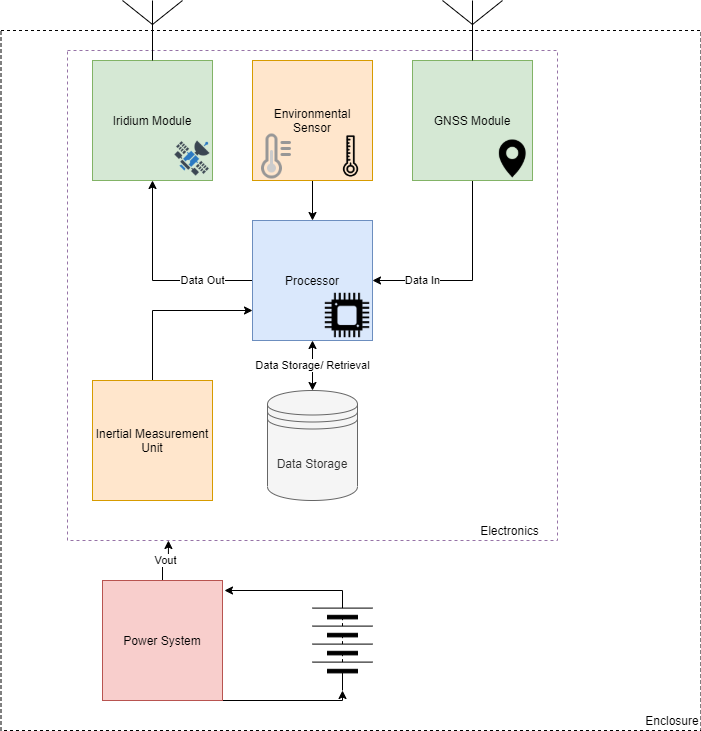
\includegraphics[width=\linewidth]{SHARC_NODE}
    \caption{Block diagram of the proposed autonomous system showing subsystem arrangement, data flow and interfaces with the environment.}
    \label{mbuoy}
\end{figure}

These subsystems can be further broken down into components requirements as shown in the figure below

\begin{figure}[H]
    \centering
    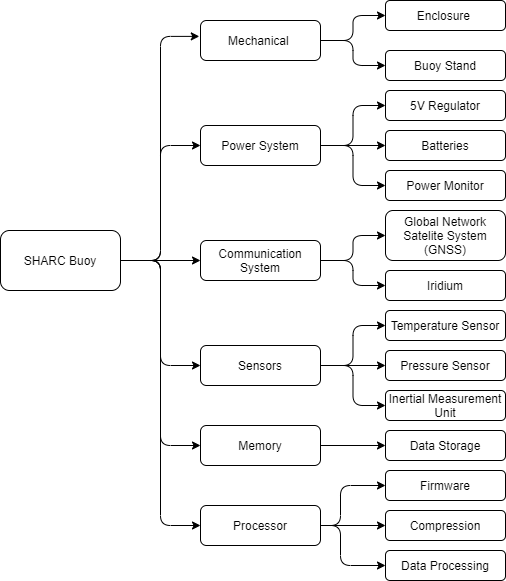
\includegraphics[width=0.8\textwidth]{Subsystem_Diagram.png}
    \caption{Breakdown of subsystems from table \ref{tab:subsys} into usable components.}
    \label{fig:ss_breakdown}
\end{figure}



\subsection{Technical specifications}

These technical specifications will be used to determine what hardware is required to construct the subsystems as showing in Figure \ref{mbuoy} above.

%%%FIX THIS TABLE

\begin{table}[H]
    \centering
    \caption{Technical specifications for the overall system}
     \setlength{\extrarowheight}{5pt}
    \resizebox{\textwidth}{!}{%
    \begin{tabular}{>{\centering\arraybackslash}m{0.25\textwidth}>{\raggedright\arraybackslash}m{0.6\textwidth} >{\raggedright\arraybackslash}m{0.35\textwidth} }
        \hline
         \textbf{Specification ID} & \textbf{Description} & \textbf{Functional requirement addressed} \\
         \hline
         \hline
         \multirow{2}{0.2\textwidth}{SP001} & \multirow{2}{0.6\textwidth}{Enclosure built using thermal resistant plastic.} & FR001\\ && FR002\\
         \hline
         \multirow{3}{0.2\textwidth}{SP002}  & \multirow{3}{0.6\textwidth}{Electronics to be mounted on a 1.5 m stand constructed from non-corrosive metal.} & FR002\\ && FR003\\ &&FR004\\
         \hline
         \multirow{1}{0.2\textwidth}{SP003} & System to include desiccant packets inside the enclosure. & FR003 \\
         \hline
         \multirow{1}{0.2\textwidth}{SP004} & Device to have a temperature operating range of $-40 ^\circ \text{ C to } 20 ^\circ$ C with $ 1^\circ$ C uncertainty. & FR009 \\
          \hline
         \multirow{1}{0.2\textwidth}{SP005}& Subsystems to be rated for $3.3 \textbf{ V to } 5$ V power. & FR008 \\
          \hline
         \multirow{1}{0.2\textwidth}{SP006}& Device shall survive for 1 month on a single set of cells & FR007 \\
          \hline
         \multirow{1}{0.2\textwidth}{SP007} & The device should cost less than R10,000 & FR016 \\
         \hline
         \multirow{1}{0.2\textwidth}{SP008} & System will contain flash chips for permanent storage. & FR012 \\
         \hline
         \multirow{1}{0.2\textwidth}{SP009}& System will use the STMicroelectronics STM32 series of microcontroller. & FR013 \\
         \hline 
         \multirow{1}{0.2\textwidth}{SP010} & The system shall be supplied by a regulated 5 V supply.  & FR014 \\
         \hline
         \multirow{1}{0.2\textwidth}{SP011} & The low power threshold occurs for voltages < 5 V & FR014 \\
         \hline 
         \multirow{4}{0.2\textwidth}{SP012}& Maximum current operations: & \multirow{4}{0.2\textwidth}{FR0014}\\
            &500 mA maximum start-up current. & \\
            &100 mA maximum active current. & \\
            &10 mA sleep current.& \\
         \hline
         \multirow{1}{0.2\textwidth}{SP013} & Device to be powered off or placed in sleep mode when inactive. & FR014 \\
         \hline
         \hline
    \end{tabular}}

    \label{tab:sys_specs}
\end{table}
\subsection{Acceptance test protocols}

In this section, the acceptance testing protocols for hardware and software modules is provided. These tests are designed to ensure that the devices meet the functional requirements outlined in table \ref{tab:hard_funcreqsl} to \ref{tab:elec_funcreqs}. A full description of the acceptance test protocols can be found in Appendix \ref{app:atp}. The goal of the acceptance criteria of each test as well as the the targeted module is given in table x below.

\begin{table}[H]
	\caption{A summary of acceptance test protocols from Appendix \ref{app:atp} showing the target and purpose of the test.}
	\label{tab:acceptance_test_summary}
	 \setlength{\extrarowheight}{5pt}
	\resizebox{\textwidth}{!}{%
		\begin{tabular}{cll}
			\hline
			\textbf{Acceptance test} & \textbf{Target} & \textbf{Purpose}\\
			\hline
			\hline
			AT001 	& Sensor modules. & Ensure module is online and functional \\
			\hline
			AT002	& All hardware modules.  & Test for faults and errors. \\
			\hline
			AT003 	& Device components. & Ensure selected components are rated for this application.\\
			\hline
			AT004	& Sensor peripheral libraries. & Verify software correctly interfaces with subsystem modules. \\
			\hline
			AT005	& Full system. & Ensuring an accelerated functional cycle meets the timing and sensing requirements. \\
			\hline
			AT006	& Sensor modules. & Calibrate the sensors against a known reference. \\
			\hline
			AT007	& Power subsystem. & Verify the power system meets the user requirements. \\
			\hline
			AT008	& Full system. & Ensure the device can operate in low temperatures. \\
			\hline
			AT009	&  Full system. & Ensure device functions in a remote environment. \\
			\hline
			\hline
		\end{tabular}
	}
\end{table}

\section{Conclusion}

To summarise, this chapter outlines the design procedure for identifying critical subsystems and technical specifications to meet the user requirements. This will provide the basis for component and module selection which will be discussed in the next chapter.

